\documentclass{article}
\usepackage[utf8]{inputenc}
\usepackage{enumitem, multicol, amsmath}
\usepackage{verbatim}
\usepackage[left=3cm, right=3cm]{geometry}
\usepackage{graphicx}
\usepackage{amssymb}
% \usepackage{pifont,eqnarray,minted}
\usepackage[ruled, vlined ,linesnumbered]{algorithm2e}
\usepackage{url}
\usepackage{fancyvrb}

\title{Inductive Logic Programming with Andante}
\author{Simon Jacquet}

\setlength{\parindent}{0pt}
\setlength{\parskip}{8pt}
\setcounter{section}{-1}

\begin{document}

\maketitle
\section{Introduction} \label{introduction}

This document is intended as documentation for the Andante python package. It 
makes the link between Inductive Logic Programming (ILP) theory and its 
implementation in the Andante toolbox.

All jupyter notebook examples can be found in the \textsc{Documentation
examples.ipynb} file in the git-repository for the Andante package at the
address: \url{https://gitlab.unamur.be/sijacque/andante/-/tree/master/src}

Section \ref{terminology} gives the terminologies used throughout the rest of 
the document and in the implementation.

Section \ref{logicProgramming} gives an overview of Logic Programming. In
particular, it describes deduction in section \ref{logicProgramming:deduction}.
Also, it describes how solving works in Logic Programming (section
\ref{logicProgramming:solver}).

Section \ref{ilp} dwelves into Inductive Logic Programming. It describes
induction in section \ref{ilp:induction}, introducing notions such as
substitution (section \ref{ilp:induction:substitution}) and clause subsumption
(section \ref{ilp:induction:subsumption}). Section \ref{ilp:inductionalgo}
gives an overview of all induction-related algorithms. Finally, section
\ref{ilp:learner} gives a few words on the Andante solver.

Section \ref{interface} introduces the Andante interface that allows for good 
understanding of the ILP learner described in the previous section.

At last, section \ref{architecture} provides the structure of the Andante
package as a whole. It regroups all modules in disctinct groups depending on
their function.

\newpage
\section{Terminology} \label{terminology}

The terminologies used in the Andante package come from various resources:
first order logic, prolog and progol. Some of those use the same terms but with
different meaning. This section aims to clarify the notions used.

Section \ref{terminology:lpconcepts} defines all terms used in the context
of Logic Programming, whereas section \ref{terminology:ilpconcepts} defines 
those used in Inductive Logic Programming.

\subsection{Logic Programming concepts} \label{terminology:lpconcepts}

Logic Programming inscribes itself in the first order logic framework. The most
well-known Logic Programming language is prolog. Alas, the terminoloy is not 
consistent in both framework. Here is described the terminology used in the 
Andante toolbox.

\begin{itemize}
    \item[\textbf{Variable:}] Universally defined variable. Implemented as
        \textsc{andante.logic\_concepts.Variable}.
        \begin{verbatim} <Variable> ::= [A-Z] [a-zA-Z_0-9]* \end{verbatim}

    \item[\textbf{Function:}] Operator that maps inputs to some output. It is
        composed of a function symbol (name beginning by a lower case) and a
        list of terms. Implemented as \textsc{andante.logic\_concepts.Function} 
        \begin{verbatim} <Function> ::= [a-z]* (<Term>, ..., <Term>) \end{verbatim}
        
    \item[\textbf{Predicate:}] Function that returns either true or false.
        Implemented as \textsc{andante.logic\_concepts.Predicate} 
        \begin{verbatim} <Predicate> ::= <Function> \end{verbatim}

    \item[\textbf{Constant:}] Function of arity 0, i.e. number or string.
        Implemented as \textsc{andante.logic\_concepts.Constant} 
        \begin{verbatim} <Constant> ::= <Number> | <String> \end{verbatim}

    \item[\textbf{Term:}] Argument of functions. Implemented as
        \textsc{andante.logic\_concepts.Term} 
        \begin{verbatim} <Term> ::= <Constant> | <Variable> | <Compound term> \end{verbatim}

    \item[\textbf{Atom:}] Atomic formula as described in first order logic.
        Implemented as \textsc{andante.logic\_concepts.Atom} 
        \begin{verbatim} <Atom> ::= <Predicate> | True | False \end{verbatim}

    \item[\textbf{Compound term:}] As defined in prolog, compound terms are any
        terms that are neither unbound variables nor atomic, i.e. constants in
        our framework. For now, compound terms only refer to functions.
        Implemented as \textsc{andante.logic\_concepts.CompoundTerm}.
        \begin{verbatim} <Compound term> ::= <Function> \end{verbatim}

    \item[\textbf{Literal:}] Atom, a.k.a. positive literal, or negation of an
        atom, a.k.a. negative literal.

    \item[\textbf{Clause:}] Finite set of literals. It is to be understood as
        the disjunction of all elements of the set. Let $A_i, B_i$ be atoms,
        the clause can be written as:
    \begin{eqnarray*}
             & \{A_1, ..., A_n, \neg B_1, ..., \neg B_m\} \\
        \iff & A_1, ..., A_n \leftarrow B_1, ..., B_m
    \end{eqnarray*}

    \item[\textbf{Horn clause:}] Clause with at most one positive literal.
        Implemented as \textsc{andante.logic\_concepts.Clause} 
        \begin{verbatim} <Horn clause> ::= <Definite clause> | <Goal clause> \end{verbatim}

    \item[\textbf{Definite clause:}] Horn clause with exactly one positive
        literal. 
        \begin{verbatim} <Definite clause> ::= <Atom> :- <Atom>, ..., <Atom> \end{verbatim}

    \item[\textbf{Goal clause:}] Horn clause with zero positive literal. 
        \begin{verbatim} <Goal clause> ::= :- <Atom>, ..., <Atom> \end{verbatim}

    \item[\textbf{Goal:}] The input to our solver. The query for which we need
        to verify the veracity. Implemented as
        \textsc{andante.logic\_concepts.Goal} 
        \begin{verbatim} <Goal> ::= (<Atom> | <Goal negation>)* \end{verbatim}

    \item[\textbf{Goal negation:}] The negation of a goal. Implemented as
        \textsc{andante.logic\_concepts.Negation} 
        \begin{verbatim} <Goal clause> ::= <Atom>, ..., <Atom> \end{verbatim}

    \item[\textbf{Logic Program}] A collection of Horn clauses. Implemented in
        \textsc{andante/knowledge.py}.  
        \begin{verbatim} <Logic program> ::= <Clause>, ..., <Clause> \end{verbatim}
\end{itemize}

\subsection{Inductive Logic Programming concepts} \label{terminology:ilpconcepts}

\begin{itemize}
    % Type
    % Mode
    % Modeh
    % Modeb

    \item[\textbf{Mode}] Mode declaration as defined in the progol framework. 
        Mode declarations define language constraints on the new clauses built 
        with Inductive Logic Programming.
        Implemented as \textsc{andante.mode.Mode}.
        \begin{verbatim} <Mode> ::= <Modeh> | <Modeb> \end{verbatim}

    \item[\textbf{Modeh}] Mode declaration for the head literal of a clause.
        Implemented as \textsc{andante.mode.Modeh}.
        \begin{verbatim} <Modeh> ::= modeh ( <Integer>, <MPredicate> ) \end{verbatim}

    \item[\textbf{Modeb}] Mode declaration for body literals of a clause.
        Implemented as \textsc{andante.mode.Modeb}.
        \begin{verbatim} <Modeb> ::= modeb ( <Integer>, <MPredicate> ) \end{verbatim}

    \item[\textbf{MPredicate}] Predicate whose terms are \textsc{MTerms}.

    \item[\textbf{MTerm}] Special Term for Mode declarations. MTerms have
        \textsc{Type} instead of \textsc{Variable}.
        \begin{verbatim} <MTerm> ::=  <Constant> | <Type> | <MCompoundTerm> \end{verbatim}

    \item[\textbf{MCompoundTerm}] Compound term whose terms are \textsc{MTerms}.

    \item[\textbf{Type}] Object used in the progol framework to tell to what
        corresponds the Type. \textsc{+} is for input Variable, \textsc{-} is
        for output Variable and \textsc{\#} is for Constant.
        The string after \textsc{+-\#} gives the class which represents the 
        Variable / Constant, e.g. a person or an animal.
        \begin{verbatim} <Type> ::=  [+-#] <String> \end{verbatim}
\end{itemize}

\subsection{Parser} \label{terminology:parser}

The terms defined above form together a grammar. The Andante package implements
a parser for each term as a single class \textsc{andante.parser.Parser}. This 
class relies on the module \textsc{andante/grammar.py} for interpreting input strings
into grammatical trees and on the module \textsc{andante/grammar\_tree\_visitor.py} to
transform those grammatical trees into python objects.

It is worth noting that the Andante parser builds upon the 
\textsc{parsimonious} python package \cite{parsimonious}.

Figure \ref{parserexample} illustrates with an example a trivial use of the 
parser.

\begin{figure}[h!]
    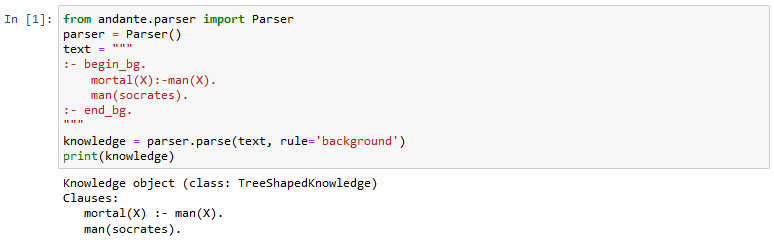
\includegraphics[width = \textwidth]{images/Parser example.PNG}
    \caption{Jupyter notebook cell showcasing the use of the Andante parser}
    \label{parserexample}
\end{figure}



\newpage
\section{Logic Programming} \label{logicProgramming}

Logic Programming is a programming paradigm that allows for computers to
reason. The most famous language upholding this paradigm is Prolog. 

Section \ref{logicProgramming:deduction} describes how one can reason through
deduction. Illustrating theory with a simple example.

Section \ref{logicProgramming:solver} presents how one uses the Andante solver,
the deduction engine.

\subsection{Deduction} \label{logicProgramming:deduction}

Deduction happens when one reasons by drawing deductive inferences, i.e. by
applying rules of inference. In Logic Programming, such rules are represented 
by Horn clauses. 

An Horn clause can be noted as:
$$ H \leftarrow B_1, \dots, B_n $$
where $H$ and $B_i$ are atoms. In Logic Programming, Horn clauses are often
noted as:
\begin{verbatim} H :- B1, ..., Bn \end{verbatim}

The rule is to be read as: if all $B_i$ are true, then $H$ is true. The rule
can also be read as: for $H$ to be true, all $B_i$ need to be true.
It is worth noting that in the case of a Goal clause, i.e. when there are no 
$H$ in the clause, the rule becomes: it can never happen that all $B_i$ are
true at the same time.
Another interesting case is when there exists no $B_i$. The rule then becomes a
fact: $H$ is true.

Of course, in general we use multiple Horn clauses to realize our deduction. 
This is where comes into action Logic Programs which are nothing more than a 
collection of Horn clauses.

Also, one may want to deduce the validity of more than a simple atom. Goals 
allows for just that.

\subsubsection*{Example} \label{logicProgramming:deduction:example}

To better understand deductive inferences, let us consider the following Logic
Program composed of two Horn clauses:
\begin{verbatim}
    C1 ::= mortal(X) :- man(X).
    C2 ::= man(socrates).
\end{verbatim}
This Logic Program tells us that (i) all men are mortals and (ii) Socrates is a
man.

Now, let us try to deduce the following goal:
\begin{verbatim}
    mortal(X).
\end{verbatim}
The question this goal asks is the following: who/what are mortal? From $C1$,
we can deduce a new goal: \Verb#man(X).#. And from $C2$, we know that the
substitution $\{X/socrates\}$ answers the initial query.

\subsection{Solver} \label{logicProgramming:solver}

Once one has defined a logic program, one can query this logic program. The 
Andante toolbox allows to do so through the \textsc{andante.solver.Solver} class.
This class provides two methods to query a logical program. The first method 
\textsc{succeeds\_on} tells whether there is a substitution for that query. The 
second method \textsc{query} gives the substitution for that query.

Figure \ref{solverexample} illustrates both methods in a simple example. This
cell is executed in a jupyter notebook after the cell presented in section 
\ref{terminology:parser}. Both \textsc{parser} and \textsc{knowledge} are
defined there.

\begin{figure}[h!]
    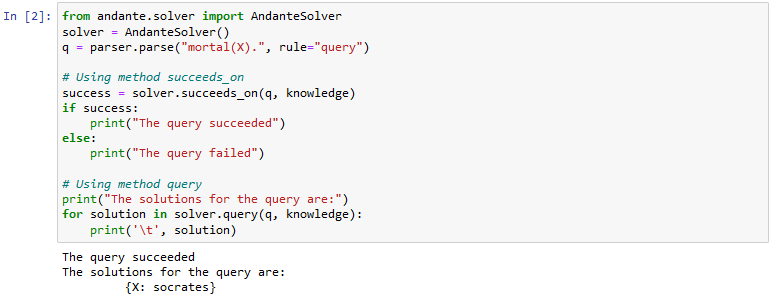
\includegraphics[width = \textwidth]{images/Solver example.PNG}
    \caption{Jupyter notebook cell showcasing both methods form the Solver 
    class}
    \label{solverexample}
\end{figure}

\newpage
\section{Inductive Logic Programming} \label{ilp}

Inductive Logic Programming (ILP) is a type of machine learning based on the
concept of induction.

Section \ref{ilp:induction} introduces the fundamentals of induction. 
Section \ref{ilp:inductionalgo} gives the progol algorithms that together form
the ILP Andante implements.
Section \ref{ilp:learner} talks about how induction is conducted in Andante.

\subsection{Induction} \label{ilp:induction}

Induction is defined as the inverse of deduction which is explained in section
\ref{logicProgramming:deduction:substitution}.

Let us look back the example from section
\ref{logicProgramming:deduction:example}.

In deduction, from prior knowledge:
\begin{center}
\begin{tabular}{lll}
    Statement A & & All men are mortal \\
\end{tabular}
\end{center}
One deduces a new fact.
\begin{center}
\begin{tabular}{lll}
    Statement B & & Socrates is mortal \\
\end{tabular}
\end{center}

In induction, from some fact:
\begin{center}
\begin{tabular}{lll}
    Statement B & & Socrates is mortal \\
\end{tabular}
\end{center}
\begin{center}
One deduces the knew knowledge:
\begin{tabular}{lll}
    Statement A & & All men are mortal \\
\end{tabular}
\end{center}

From this example, one fact is important to notice.
Deduction is an sound operation in the sense that if the prior knowledge is
correct, the deduced fact is always correct. Induction is not a sound
operation. Even if the fact(s) it is based on is (are) true, the induced
knowledge may not be correct.

Deduction is making inferences from a general knowledge to a specific instance.
Induction is generalizing specific instances into a general knowledge.
In the examples provided above, statement A is indeed more general than
statement B.
To give a more rigorous explanation of the concept of generality, we first need
to introduce the notions of substitution and subsumption.

\subsubsection{Substitution} 
\label{ilp:induction:substitution}

Let $\theta$ be a substitution of the form \{$v_1/t_1, ..., v_n/t_n$\}. Let $F$
be an arbitrary formula. We note: 
$$F' = F\theta$$ 
where $F'$ is the formula $F$ with each variable $v_i$ of $F$ that is also a
variable of $\theta$ has been replaced by $t_i$.

Substitution is implemented in Andante as the class
\textsc{andante.substitution.Substitution}. This class handles:
\begin{itemize}
    \item Unification with its method \textsc{unify}
    \item Substitution with its method \textsc{substitute}
\end{itemize}

\subsubsection{Clause subsumption}
\label{ilp:induction:subsumption}

Let $C$ and $D$ be clauses. We say that $C$ subsumes $D$, that is:
$$C \preceq D \iff \exists \theta, C\theta \subseteq D$$

Using subsumption, we now have a rigorous method to tell whether a clause $C$
is more general than another clause $D$ by testing if $C$ subsumes $D$.

Taking back the examples from section \ref{ilp:induction}, as statement A
subsumes statement B, we can say that deduction goes from general to specific 
and induction goes from specific to general.

\subsection{Induction algorithm} \label{ilp:inductionalgo}

This section describes the method used for using induction to learn new
knowledge. The learning process of Andante closely follows that of progol. It
is composed of three algorithms described in sections
\ref{ilp:inductionalgo:coverset}, \ref{ilp:inductionalgo:bottomi} and
\ref{ilp:inductionalgo:latticesearch}. Lastly, section
\ref{ilp:inductionalgo:metrics} introduces all metrics related functions used
in section \ref{ilp:inductionalgo:latticesearch}.
% TODO: insert reference

\subsubsection{Cover set alogorithm} \label{ilp:inductionalgo:coverset}

The first and main algorithm which glues together the three algorithms is the
Cover set algorithm (see \ref{algo:coverSet}). It iterates through all positive
examples, constructing a theory that covers all positive examples whilst never
covering any negative ones. The Andante implementation of this algorithm can be
found as the \textsc{induce} method of the \textsc{andante.learner.ProgolLearner}
class.

\begin{algorithm}[H]
\label{algo:coverSet}
\caption{Cover set algorithm}
\SetKwInOut{Input}{input}
\Input{$h,i,B,M,E$}
If $E = \emptyset$ return $B$ \\
Let $e$ be the first example in $E$ \\
Construct clause $\bot_i$ for $e$ \tcp*{Algorithm 2}
Construct clause $H$ from $\bot_i$ \tcp*{Algorithm 3}
Let $B = B \cup H$ \\
Let $E' = \{e: e \in E \text{ and } B \models e\}$ \\
Let $E = E-E'$ \\
Goto 1
\end{algorithm}

\subsubsection{Algorithm for $\bot_i$} \label{ilp:inductionalgo:bottomi}

For each new clause added to the theory, it is first necessary to construct a 
more specific clause called $bot_i$. This is precisely the role of algorithm
\ref{algo:constructboti}. This algorithm is implemented in the 
\textsc{build\_bottom\_i} method of the \textsc{andante.learner.ProgolLearner}
class.

\begin{algorithm}[H]
\label{algo:constructboti}
\caption{Algorithm to construct $\bot_i$}
\SetKwInOut{Input}{input}
\Input{$h,i,B,M,E$} % TODO
Add $\overline{e}$ to the background knowledge \\
$InTerms = \emptyset$, $\bot_i = \emptyset$ \\
Find the first head mode declaration $h$ such that $h$ subsumes $a$ with 
substitution $\theta$ \\
\ForAll{$v/t \in \theta$}{
    \lIf*{$v$ corresponds to a \#type}{replace $v$ in $h$ by $t$} \\
    \If{$v$ corresponds to a +type or -type}{
        replace $v$ in $h$ by $v_k$ \\
        where $v_k$ is the variable such that $k = hash(t)$ \\
    }
    \lIf*{$v$ corresponds to a +type}{add $t$ to the set $InTerms$} \\
}
Add $h$ to $\bot_i$ \\
\ForAll{body mode declaration $b$}{
    \ForAll{possible substitution $\theta$ of variables corresponding to +type by terms from the set InTerms}{
        \Repeat{recall times}{
            \If{Progol succeeds on goal $b$ with answer substitution $\theta'$}{
                \ForEach{$v/t$ in $\theta$ and $\theta'$}{
                    \lIf{$v$ corresponds to \#type}{
                        replace $v$ by $b$
                    }
                    \lElse{
                        replace $v$ in $b$ by $v_k$ where $k = hash(t)$
                    }
                    \lIf{$v$ corresponds to -type}{
                        add $t$ to the set InTerms
                    }
                }
                Add $\overline{b}$ to $\bot_i$
            }
        }
    }
}
Increment the variable depth \\
Goto line 11 if the maximum variable depth has been achieved
\end{algorithm}

\subsubsection{Lattice search algorithm} \label{ilp:inductionalgo:latticesearch}

Once the most specific (because of its long boy) clause $\bot_i$ is 
constructed, we can now compare various possible clauses to add to our previous
knowledge. This is the role of algorithm \ref{algo:latticeSearch}. It can be 
found as the \textsc{build\_hypothesis} method of the 
\textsc{andante.learner.ProgolLearner} class.

\begin{algorithm}[H]
\label{algo:latticeSearch}
\caption{Lattice search algorithm}
\SetKwInOut{Input}{input}
\Input{$h,i,B,M,E$}
$Open = \{\square\}$, $Closed = \emptyset$ \\
$s = best(Open)$, $Open = Open - s$, $Closed = Closed \cup \{s\}$  \tcp*{Node selection}
\lIf*{$prune(s)$}{goto 5  \tcp*{Node pruning}} 
$Open = (Open \cup \rho(s)) - Closed$ \tcp*{Clause refinement}
\lIf*{$terminated(Closed, Open)$}{\Return $best(Closed)$ \tcp*{End of search}}
\lIf*{$Open = \emptyset$}{\Return $e$\tcp*{No generalisation}} 
Goto 2
\end{algorithm}

\subsubsection{Metrics for the lattice search algorithm} \label{ilp:inductionalgo:metrics}

There can be multiple variations of this algorithm. For instance, depending on
whether we have access to negative examples, the notion of best or terminated
will be different.
In total, there are four functions whose definition may change: best, prune,
$\rho$, terminated.

The Andante toobox implements only the case where we have access to both
positive and negative examples. All those functions are implemented in the
\textsc{andante.hypothesis\_metrics.py} module.

\begin{itemize}
    \item Let $s$ be the current state. 
    \item Let $C$ be the clause of state $s$.
    \item Let $p$ be the number of positive examples rightly covered by $C$.
    \item Let $n$ be the number of negative examples wrongly covered by $C$.
    \item Let $c$ be the number of elements in the body of $C$.
    \item Let $d$ be a function giving an optimistic estimate of the number of
        atoms needed to complete the clause.
            \[
                d(C) = \max_{v \in C_{body}} d(v) \\
                d(v) = 
            \begin{cases}
                0, & \text{if } v \text{is in the head of }C\\
                (\max_{u\in U_v} d(u)) +1,              & \text{otherwise}
            \end{cases}
            \] where $U_v$ are the variables in atoms in the body of $C$ containing $v$.
    \item Let $h$ be $d(C)$.
    \item $g = p-c-h$
    \item $f = g-n = p-n-c-h$
\end{itemize}

\subsection{Learner} \label{ilp:learner}

In the Andante package, the ILP learning is done through the 
\textsc{andante.learner.Learner} class. This class is used through the induce
method which produces a the knowledge learned through ILP.

Figure \ref{learnerexample} illustrates on a simple example the learning. The 
cell follows the execution of the cells presented in figures 
\ref{parserexample} and \ref{solverexample}. In particular, \textsc{parser} is
defined there.

\begin{figure}[h!]
    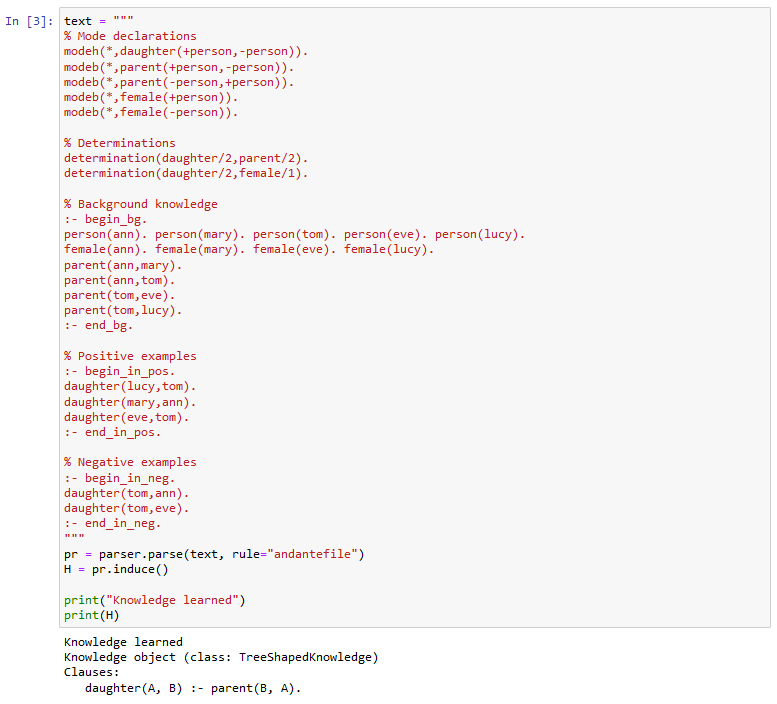
\includegraphics[width = \textwidth]{images/Learner example.PNG}
    \caption{Jupyter notebook cell showcasing learning on a simple example}
    \label{learnerexample}
\end{figure}

\section{Interface} \label{interface}

Inductive Logic Programming can come as quite cryptic when first glanced at.
The documentation available is often not sufficient to understand precisely
what is going on. To this purpose, the Andante Interface provides a great way
to view in a more intuitive way the learning process. The Andante Interface is
implemented in the \textsc{andante/interface.py} module. It relies on the
\textsc{ipywidgets} library\footnote{Source:
\url{https://ipywidgets.readthedocs.io/en/stable/}} to provide panels formed
from those widgets that the user can interact with.

The Andante Interface comes in 3 panels (figures
\ref{fig:interface:querypanel}, \ref{fig:interface:detailspanel} and
\ref{fig:interface:inducepanel}).

The Andante Interface (see \textsc{andate.interface.MainInterface}) provides a
panel for querying knowledge (see \textsc{andate.interface.QueryInterface}). In
figure \ref{fig:interface:querypanel}, we see that for the query
\textit{mother(sylvia, X).}, there are 4 possible substutions.

\begin{figure}[h!]
    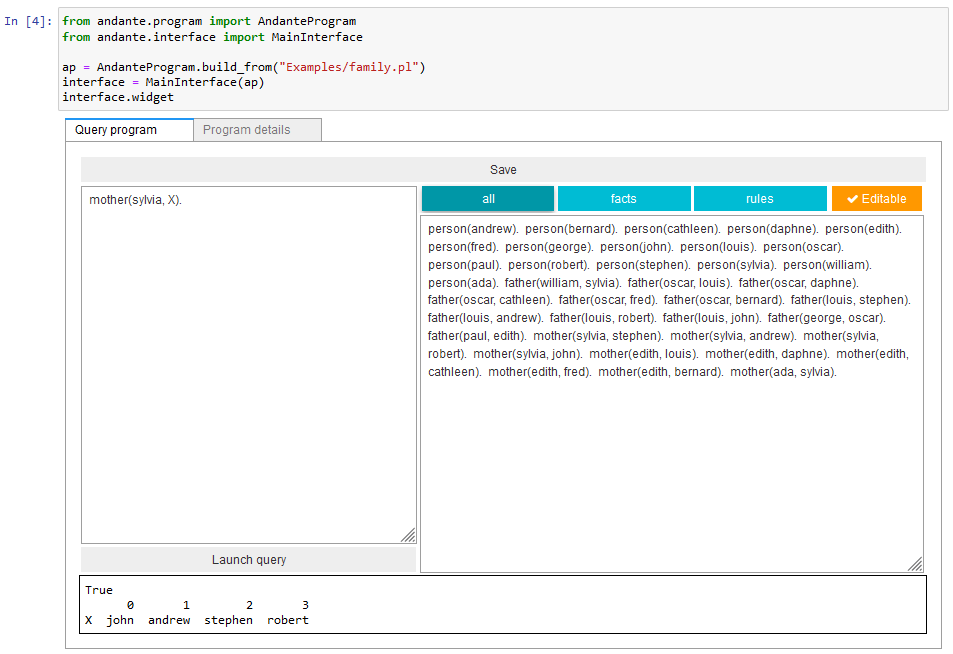
\includegraphics[width = \textwidth]{images/Interface - query results.PNG}
    \caption{Query panel of the Andante Interface}
    \label{fig:interface:querypanel}
\end{figure}

The second panel (see \textsc{andate.interface.DetailsInterface}) shown in
figure \ref{fig:interface:detailspanel} shows numerous details on the
\textsc{AndanteProgram} considered. All those details can be edited. The button
\textit{Induce} launches the learning process and opens a new panel.

\begin{figure}[h!]
    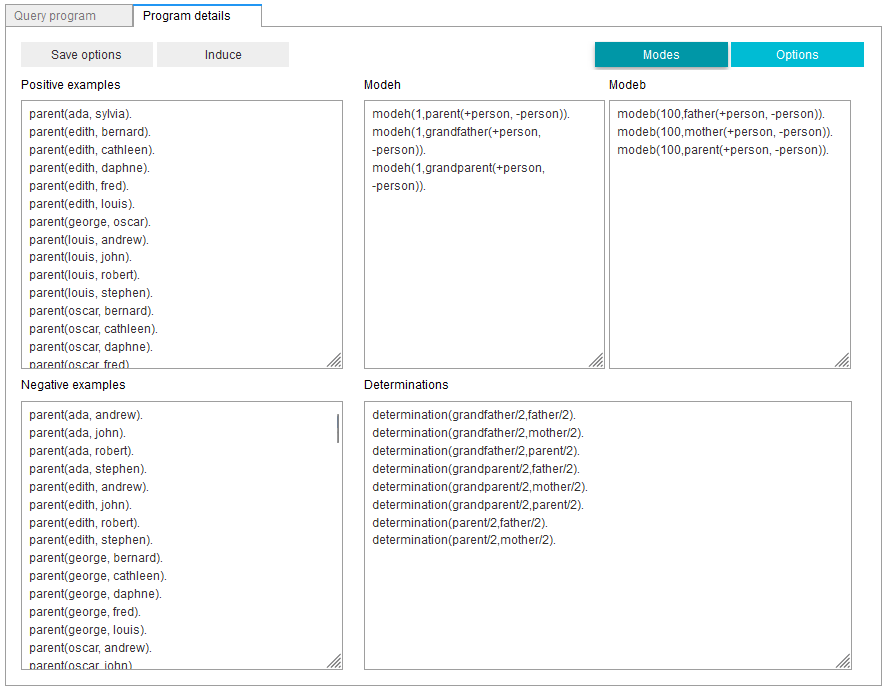
\includegraphics[width = \textwidth]{images/Interface - details.PNG}
    \caption{Program details panel of the Andante Interface}
    \label{fig:interface:detailspanel}
\end{figure}

The last of the major panels is the \textit{Induction} panel (see
\textsc{andate.interface.DetailsInterface}), as shown in figure
\ref{fig:interface:inducepanel}. When first opened, this panel offers many
details on the learning process that can be played with. In particular, for a
particular example, one can find: the bottom clause and all candidate clauses.
For a candidate clause, one can find all positive and negatvie examples it
covers. In figure \ref{fig:interface:inducepanel}, one can see for the rule
\Verb#parent(A, B):- mother(A, B).# all the covered positive examples.

\begin{figure}[h!]
    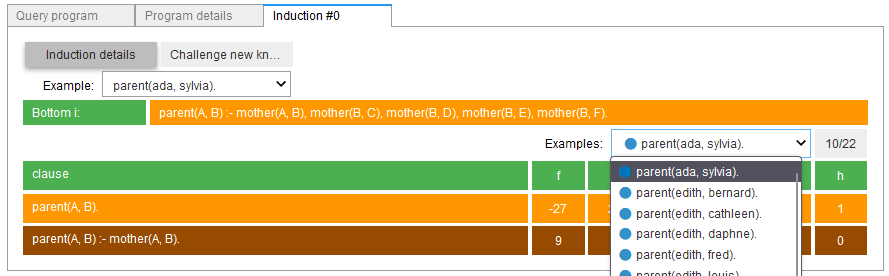
\includegraphics[width = \textwidth]{images/Interface - induction - examples.PNG}
    \caption{Induce panel of the Andante Interface}
    \label{fig:interface:inducepanel}
\end{figure}

A subpanel (see \textsc{andate.interface.QueryInterface}) of this last panel is
shown in figure \ref{fig:interface:queryinducedpanel}. In this panel, one can
challenge the knowledge both before and after induction.

\begin{figure}[h!]
    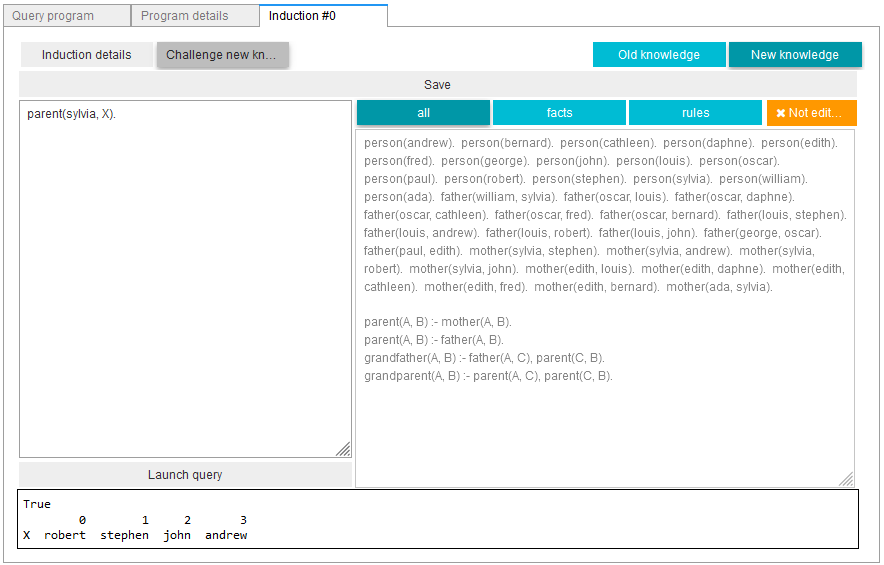
\includegraphics[width = \textwidth]{images/Interface - induction - query.PNG}
    \caption{Query panel for the induced knowledge of the Andante Interface}
    \label{fig:interface:queryinducedpanel}
\end{figure}

\section{Package architecture} \label{architecture}

\begin{itemize}
    \item \textbf{Utilities:} Regroups a few utility classes.
    \begin{itemize}
        \item \textsc{collections.py}: Defines \textsc{OrderedSet} class.
        \item \textsc{options.py}: Option-related classes.
    \end{itemize}
    
\item \textbf{Basic objects:} Regroups all classes implementing terminology
    as described in section \ref{terminology:lpconcepts}.
    \begin{itemize}
        \item \textsc{logic\_concepts.py}: Classes for Logic Concept terminology
            as described in section \ref{terminology:lpconcepts}.
        \item \textsc{mode.py}: Classes for Inducive Logic Concept terminology
            as described in section \ref{terminology:ilpconcepts}.
        \item \textsc{mathematical\_expressions.py}: Classes for all
            mathemitical expressions.
        \item \textsc{knowledge.py}: Classes that act as knowledge, i.e.
            collections of clauses.
    \end{itemize}
    
    \item \textbf{Parsing:} Regroups modules for parsing text into Python
        objects.
    \begin{itemize}
        \item \textsc{grammar.py}: Module for defining the grammar for parsing.
            The class also allows to transform text into a grammar tree.
        \item \textsc{grammar\_tree\_visitor.py}: Module for turning the grammar
            tree into Python objects.
        \item \textsc{parser.py}: Main module for parsing text. It makes the
            link between the two previous modules.
    \end{itemize}
    
    \item \textbf{Solving:} Regroups modules around the engine for deduction.
    \begin{itemize}
        \item \textsc{substitution.py}: Defines the \textsc{Substitution} class
            that handles substitution but also unification.
        \item \textsc{solver.py}: Implements the engine for deduction.
    \end{itemize}
    
    \item \textbf{Learning:} Regroups modules around the induction engine.
    \begin{itemize}
        \item \textsc{hypothesis\_metrics.py}: Metrics for choosing the best
            clause to learn.
        \item \textsc{learner.py}: Engine for induction, i.e. learning new
            clauses.
        \item \textsc{live\_log.py}: Logs for storing information produced by
            the induction engine.
    \end{itemize}
    
    \item \textbf{Interface:}
    \begin{itemize}
        \item \textsc{interface.py}: Defines interfaces to query, induce,
            inspect an Andante program.
    \end{itemize}
    
    \item \textbf{Program:}
    \begin{itemize}
        \item \textsc{program.py}: Defines the \textsc{AndanteProgram} class
            that facilitates using the paser, the solver and the learner.
    \end{itemize}
    
\end{itemize}


\bibliographystyle{plain}
\bibliography{source}

\end{document}
